%This fixes a weird error I don't understand
\RequirePackage{ifluatex}
\let\ifluatex\relax

\documentclass[11pt]{article}
\author{Yohan Lefol, Marie Terrien, Alexis Dupis, and Ugo Vidal}

\title{
\textsc{User Guide}\\[2.6cm]
{\LARGE \bfseries CelloMap}
}

\author{
Yohan Lefol
\and 
Alexis Dupis
\and
Ugo Vidal
\and
Marie Terrien
}

\date{
\today
}


\usepackage{hyperref}
\usepackage{graphicx}
\usepackage{apacite}
\usepackage[margin=3cm]{geometry}
\usepackage{comment}
\usepackage[english]{babel}
\usepackage{titlesec}
\usepackage{setspace}
\usepackage{mwe}
\usepackage[utf8]{inputenc}
\usepackage{listings}
\usepackage{color}

%Numbering of pages in bottom right
\usepackage{scrpage2}
\ifoot[]{}
\cfoot[]{}
\ofoot[\pagemark]{\pagemark}
\pagestyle{scrplain}

\usepackage[acronym,nomain,toc,section=section]{glossaries}
\loadglsentries{acronyms}
\makeglossaries

%Set up to write code in the document
\definecolor{dkgreen}{rgb}{0,0.6,0}
\definecolor{gray}{rgb}{0.5,0.5,0.5}
\definecolor{mauve}{rgb}{0.58,0,0.82}

\lstset{frame=tb,
  language=R,
  aboveskip=3mm,
  belowskip=3mm,
  showstringspaces=false,
  columns=flexible,
  basicstyle={\small\ttfamily},
  numbers=none,
  numberstyle=\tiny\color{gray},
  keywordstyle=\color{blue},
  commentstyle=\color{dkgreen},
  stringstyle=\color{mauve},
  breaklines=true,
  breakatwhitespace=true,
  tabsize=3
}

\setcounter{secnumdepth}{4}

\begin{document}
\maketitle
\hrule
\begin{center}

\includegraphics[width = 8cm]{logo-CELLOMET-a.png}
\end{center}

\begin{center}

\includegraphics[width = 7cm]{Logo-Master-GPhy.png}
\end{center}
\thispagestyle{empty}


\tableofcontents


\newpage
\section{Introduction \label{intro}}
The non-canonical analysis tool (CelloMap) is a tool with several uses. Its main feature is a non-canonical gene analysis. Yet this tool also boasts several other interesting functionalities such as differential expression analyses, customizable MA and Volcano plots. Customized figures allow users to extract the significant genes (according to their own parameters) from the plots, among these, the volcano plot offers the best solution for significance as it measures p-value vs log2FoldChange. Additionally, this tool is also capable of converting gene symbols to \acrshort{KEGG} identifier (type \acrshort{hsa}), see \autoref{gene_list_analysis} for more information.
This guide will go over each functionality and explain how to best use CelloApp.

As can be seen in \autoref{fig:main_app_screen}, the application is split into several tabs. The information tab shows the user guide pdf file. The last tab `Citation' is a simple tab which gives the citation information for the use of this tool. This guide will now go over the remaining tabs and explain their uses and functionalities.
\begin{figure}[h!]
\centering
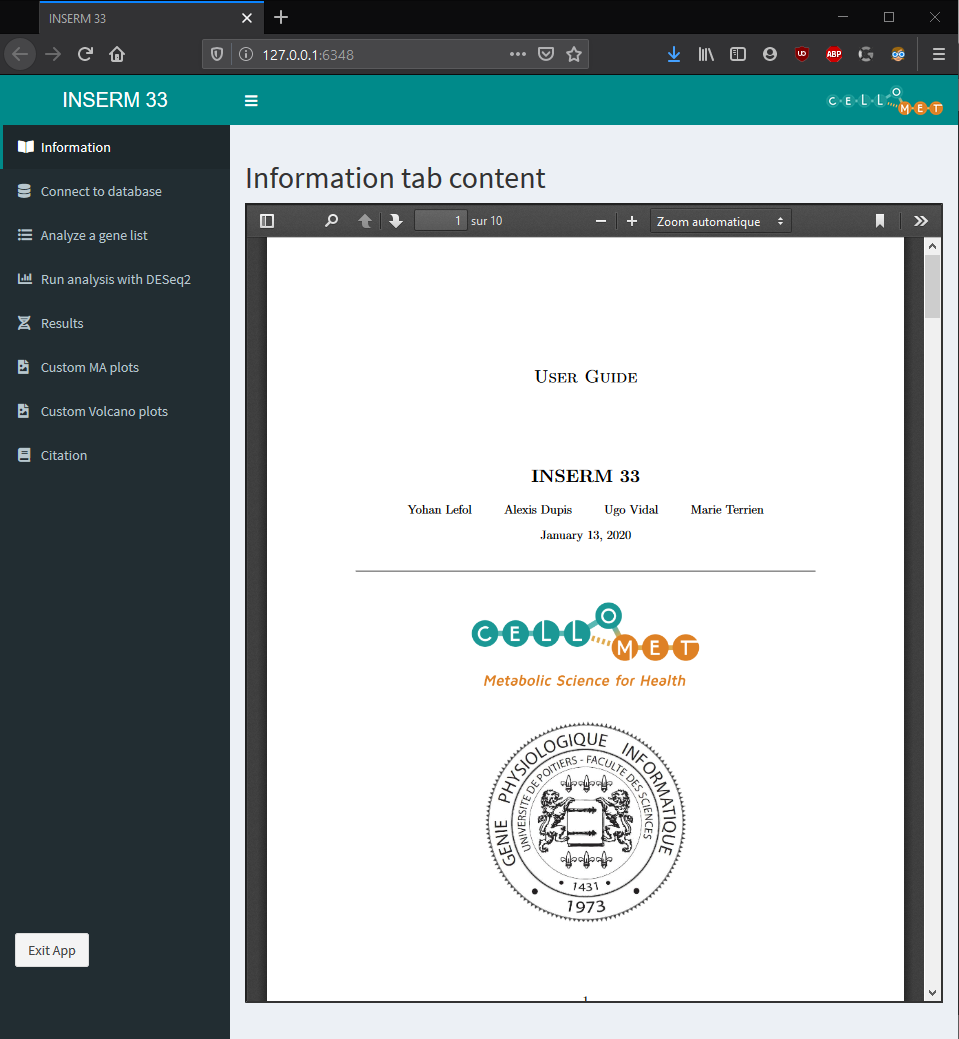
\includegraphics[width=15cm,height=10cm,keepaspectratio]{main_app_screen.png}
\caption{The main tab for the application.}
\label{fig:main_app_screen}
\end{figure}

\section{Installation \label{install}}
To launch a shiny application locally (which is the objective) our options are limited. Currently we have two methods to use the application on windows and one to use it on Mac.
The reason that windows has two methods is in case users are lacking administrative privileges on their computers preventing them from running bat files. However the second option requires more downloads than the first.\\
Basically, for Windows we managed to package everything into one folder, thus no other downloads are required, however this only works using bat files. The entire process is explained in \autoref{win_1}.
If this solution doesn't suit a user, we have an alternative solution. The alternative is to download R and R studio, and run the code manually. This is not a complicated thing, however it does require that the user downloads and installs two extra programs. This is further explained in \autoref{alter_install}.\\
The installation for Mac is nearly identical to the alternate Windows solution, it too is further explained in \autoref{alter_install}.
\subsection{Windows first solution\label{win_1}}
In order to package the application into a executable file, we used a tool called R portable \cite{R_portable} with the solution called `DesktopDeployR' \cite{Deploy_R_Shiny}. This solution allowed us to combine R, the various packages we used, and the code for the application into one folder. In order for a user to install this version of our application, he must only download the folder and launch the application using the `CelloMap.bat' file. Standard windows computers will raise a warning when a .bat file is clicked, to continue you must allow the computer to read the script.\\
In order to put some minds at ease, an explanation of the entire launch process will be given below.\\
A bat file (short for batch file) is a type of script file used by windows to execute a series of commands within the command line interpreter. The code used in our bat file is the following:
\lstset{language=C++}
\begin{lstlisting}
	wscript dist\script\wsf\run.wsf
\end{lstlisting}
Let's break this down. First we see wscript, this is a command that allows us to call another script of a different programming language, in our case we are using it to call a javaScript file. Next we see the path (dist\textbackslash script\textbackslash wsf\textbackslash run.wsf) this is the location of the next file that will be executed (run.wsf). This file contains the following code:
\lstset{language=Java}
\begin{lstlisting}
	<job id="IncludeExample">
   		<script language="JScript" src="js/json2.js"/>
   		<script language="JScript" src="js/JSON.minify.js"/>
   		<script language="JScript" src="js/run.js" />
	</job>
\end{lstlisting}
This \acrshort{wsf} (Windows Script File) allows us to launch three seperate javascript files. These files are used to configure the launch options. Simply put, the first file (json2.js) allows us to restructure our files and create the skeleton for the application, the minify.js file ensures that comments in the code are not read as code, and finally run.js calls the run.R script.\\
The run.R script then calls the app.R script which will `fill' the application with the intended content (our application).\\
If there are any concerns concerning the installation, feel free to check the webpage of DesktopDeployR \cite{Deploy_R_Shiny}. If concerns remain afterwards, feel free to use the alternate solution or contact one of the developers at: yohan.lefol@gmail.com.

\subsection{Alternative (Mac and Windows)\label{alter_install}}
As mentionned above, the alternative solution is to download R and R studio. What this means is that the user must download the programming language (R) and the \acrshort{IDE} (Integrated Development Environment) in order to run the code that he will have downloaded from the website \cite{Cellomet}.
\begin{enumerate}
\item \textbf{Download R}\\
First you will want to download the latest version of R from the following website: \url{https://www.r-project.org/}
\\Version 3.6.2 was used to develop this application.

You will have to select a `CRAN mirror', select the region from which you are working, if there are several links for your region, select one, the choice does not matter.\\
Now select the download necessary for your work station (Windows, Mac or Linux) and follow the download steps, leave all the parameters as default.
\item \textbf{Download R studio}\\
To be able to properly run the app, r studio is also required. RStudio is an IDE (Integrated Development Environment) which normally aids in maximizing a programmers productivity. For our purposes, RStudio will be used to launch the application in a browser. As with R, downloading the latest version is recommended. Version 1.2.5 was used for this application.

R Studio website: \url{https://rstudio.com/products/rstudio/download/}
\\

You will only have to select the version for your operating system (Windows, Mac or Linux) and follow the download steps, leave all the parameters as default.
\item \textbf{Download the scripts}\\
If it is not already done, download the folder containing the scripts from the Cellomet website \cite{Cellomet}.
Store the folder wherever you would like. Now you have everything you need to run CelloMap.

\item \textbf{Run the app}
You will need to open the file called `launcher.R' with Rstudio, then launch the app by highlighting(selecting) the code and pressing cmd+enter if you are on Mac, or ctrl+enter if you are on Windows.\\
\textbf{IMPORTANT: you must initiate the downloads by highlighting the text and running it. Otherwise certain packages will NOT be downloaded properly.} If this is not done properly the first time, it's not a problem, just try again using the `highlight code' method.\\
During the installation of the various packages, there will be a few pop ups asking if you want to download a package from source, always say yes to these pop-ups. The entire package set-up takes around 20-30 minutes, but it only has to be done the first time the application is launched on the computer.\\
If there are any issues concerning the download of the packages, feel free to contact Yohan Lefol using the following e-mail address: yohan.lefol@gmail.com.

\end{enumerate}


\section{Connection to database}
The identification of non-canonical genes is the main aspect of this tool. Since the list of non-canonical genes is increasing as discoveries are being made, we could not `hard code' a list of genes in the program as we wanted to ensure that the search list is being updated without having users re-download the application for each update. Therefore we implemented a database that can be updated by the owners of the tool (Cellomet) and that can be accessed remotely through this application.
In order to establish this connection, a user needs to fill in the small questionnaire as seen in \autoref{fig:connect_DB}, and click the `Connect to database' button. The answers written in the questionnaire are saved to Cellomet's database once the connection is established.

\begin{figure}[h!]
\centering
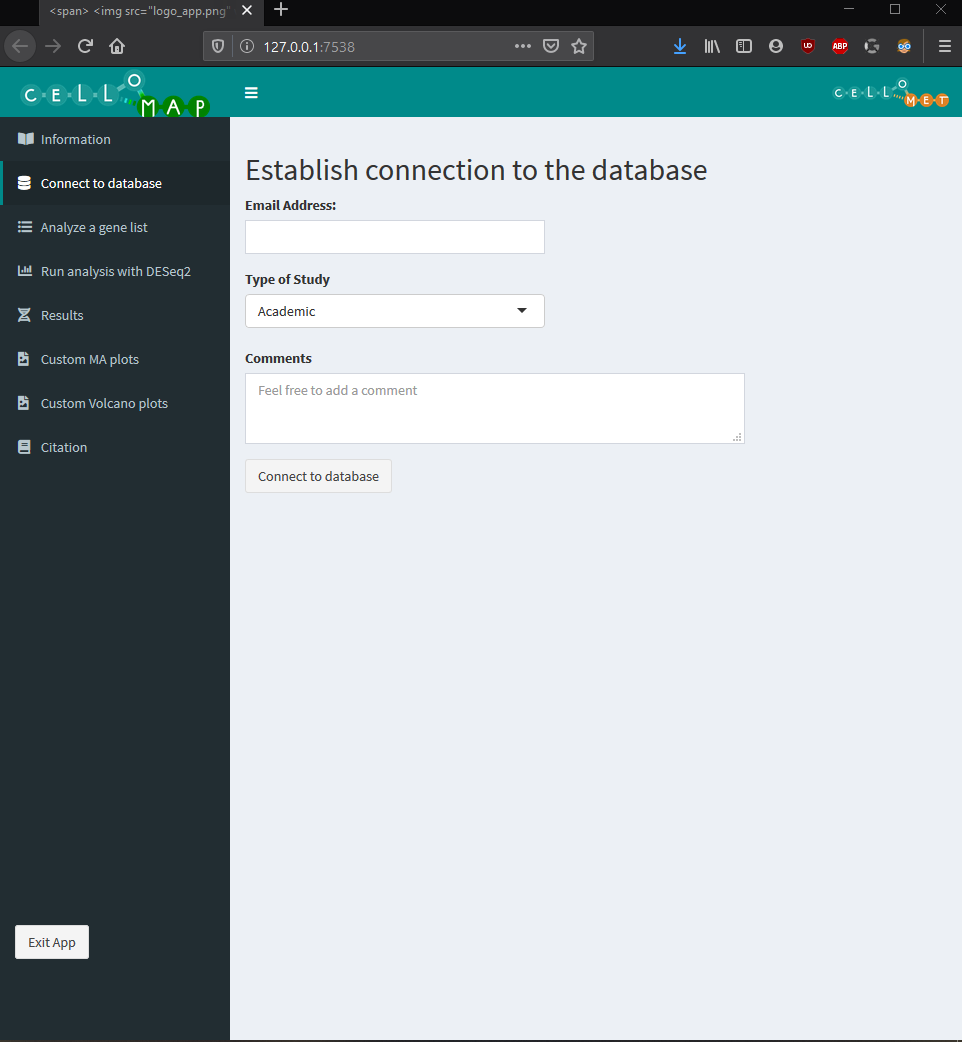
\includegraphics[width=15cm,height=10cm,keepaspectratio]{connect_DB.png}
\caption{The connect to database tab of the application.}
\label{fig:connect_DB}
\end{figure}

The database connection is only necessary if a non-canonical gene analysis or \acrshort{hsa} conversion is to be performed, either individually or as part of a \acrshort{DESeq2} analysis. If this is not the users intentions, a connection to the database is not necessary.

\section{DESeq2 analysis}
\acrshort{DESeq2} is a powerfull tool which allows users to perform differential analyses using RNAseq `COUNTS' data \cite{love2014moderated}. However this tool requires a very specific data format. This part of the guide will go over the data format necessary to run a \acrshort{DESeq2} analysis, the added parameters specific to this application, and the results that are generated.

\subsection{Tab layout \label{deseq2_layout}}
As seen in \autoref{fig:deseq2_screen}, there are several requirements for the \acrshort{DESeq2} analysis. First we observe that two files representing the two conditions that will be analyzed are required. We then observe a small check box which asks if the user want to perform a non-canonical gene analysis. Checking this box also enables the possibility of checking the \acrshort{hsa} conversion box. If the non-canonical analysis box remains checked, the user will have to be connected to the database and the non-canonical gene analysis will be run with the list of significant genes isolated by the \acrshort{DESeq2} analysis (explained below). A user can also select a directory, a directory is the location on your computer where the files will be saved.
There are then two text boxes which can be customized and are used to name the files that will be produced by the analysis. Condition 1 represents File 1 and Condition 2 represents File 2.
Lastly there are two check boxes for the creation of the standard MA and Volcano plots. If checked, two types of each plot will be made, one type with text, and the other without text. The plots generated will be with standard parameters, however a user will be able to take the differential expression data obtained from the \acrshort{DESeq2} analysis and make his own customized MA and Volcano plots with the custom plot tabs, see \autoref{custom_plots} for more details.

\begin{figure}[h!]
\centering
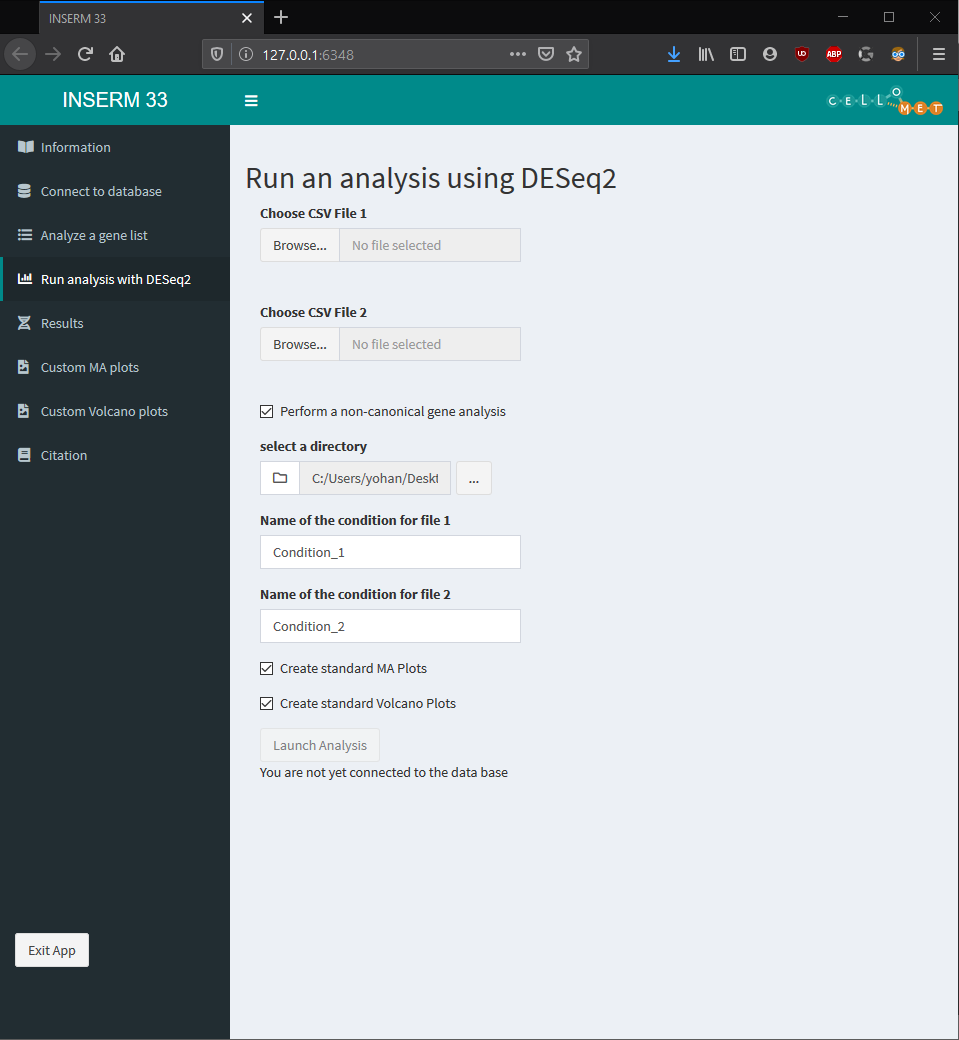
\includegraphics[width=15cm,height=10cm,keepaspectratio]{deseq2_screen.png}
\caption{The main screen for the \acrshort{DESeq2} analysis tab.}
\label{fig:deseq2_screen}
\end{figure}

\subsection{Data format \label{deseq2 data_format}}
As previously stated, \acrshort{DESeq2} requires a specific data format. We will be using \autoref{fig:data_format_deseq2} to explain the format.
This format is presented as a \acrshort{csv} file, meaning a comma separated values file, or more simply put, a file in which the different elements/values are separated by a comma.
In order to better explain the data format and what a \acrshort{csv} file really is, an excel representation of \autoref{fig:data_format_deseq2} has been created and is shown in \autoref{fig:data_format_deseq2_simplified}

\begin{figure}[h!]
\centering
\fbox{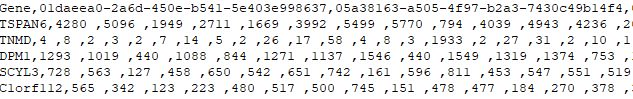
\includegraphics[width=15cm,height=10cm,keepaspectratio]{data_format_deseq2.PNG}}
\caption{The data format for a \acrshort{DESeq2} analysis.}
\label{fig:data_format_deseq2}
\end{figure}

When comparing both \autoref{fig:data_format_deseq2} and \autoref{fig:data_format_deseq2_simplified} we can clearly observe that the commas create the `separation' of the values. 
The first column represents the genes and it is important to note that these genes are in gene symbols and not another type of format such as Ensembl. \acrshort{DESeq2} will perform the analysis regardless of the type of gene name used however \textbf{a non-canonical gene analysis can only be performed with gene symbols}. As such it is advised to use gene symbols in the data in order to fully benefit from this tool. Next we have the other columns which represents the different patients. In this example, the second column shows the RNAseq `COUNTS' results of patient \#1 and the third column shows the same but for patient \#2.
\begin{figure}[h!]
\centering
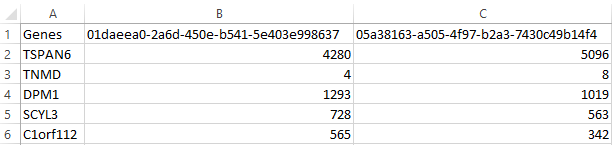
\includegraphics[width=15cm,height=10cm,keepaspectratio]{dese2_excel_data_format.png}
\caption{A simplified view of the \acrshort{DESeq2} data format.}
\label{fig:data_format_deseq2_simplified}
\end{figure}

As previously mentioned, two files are necessary, i.e: one file per condition. An easy example to explain this would be the comparative study of young vs old pulmonary cancer patients. In order to do such an analysis, we would have file \#1 contain all of the patients in the `young' category and file \#2 would contain all the patients of the `old' category. Of course both files must respect the data format. This means that both files will require the `Genes' column and both must be in the same order of gene apparition.

\subsection{launching the analysis}
Once all necessary files have been uploaded, a user can click the `launch analysis' button, at which point a pop-up will appear indicating that the analysis is being performed. This pop-up will lock the application preventing any further use, to avoid the application from crashing if too many actions are performed at once.
It is important to note that a \acrshort{DESeq2} analysis can be very quick just as it may take several hours. The length of the analysis depends on the size of the files used as well as the computing strength of the user's computer. For an old computer, it is advised to let the computer run the analysis without doing anything else on the side.\\
If an error occurs during the analysis, a error pop-up will appear and the user can obtain information about the error in the error\_log.txt that was created. Using the information from the error log, the user should consult \autoref{common_err} in order to solve the issue.\\
Once the analysis is done and if no error has occurred, the pop-up message will be replaced by a different pop-up message indicating that the analysis is done, the pop-up message will also remind the user of the location of the results.
\subsection{Results obtained}
Several results can be obtained from this analysis, some are obtained regardless of user input, others will only appear if a user has asked for those results to be generated.
\subsubsection{Main results}
A \acrshort{DESeq2} analysis generates three standard results:
\begin{itemize}
\item diffexpr\_results condition\_1 vs condition\_1 .csv\\
A differential expression file, this is a file that will contain the baseMean, log2FoldChange, \acrshort{lfcSE}, stat(used for null hypothesis test), pvalue and \acrshort{Padj} for each genes in the original files.
\item condition\_1vscondition\_1\_RESULTS\_VOLCANO.csv\\
A differential expression file for the significant genes.
\item gene\_list\_ condition\_1 vs condition\_1 \_Most\_Significant.txt\\
A list of the significant genes obtained.
\end{itemize}

It is important to note that the significant genes were obtained by filtering the main differential expression file for standard significance parameters while using a volcano plot to visualize the significant genes. The standard significance algorithm is the following:
\[\acrshort{Padj}<0.05 \ \&\ abs(log2FoldChange)>2\]
This equation indicates that genes which have a \acrshort{Padj} value below 0.05 and a log2FoldChange above 2 or below -2 are considered to be significant. A user can also generate his own list of significant genes by modifying these parameters (significant p-value and log2FoldChange threshold) in the custom volcano plot tab. This is further explained in \autoref{custom_plots} of this guide.

\subsubsection{Figures generated}
If a user has selected that he wanted standard MA and Volcano plots, there will be four png files in the results folder: Two MA plots, one with text and the other without text, and two volcano plots, one with text and one without text.
The plots with texts are much larger in order to accommodate for the additional text next to the points representing significant genes.
If a user wishes to modify these plots and create his own set, it can be easily be done in the custom plot tabs, further explained in \autoref{custom_plots} of this guide.

\subsubsection{Non-canonical gene analysis}
When a user selects a non-canonical gene analysis, there will be three extra text files in the results folder. That is, if any non-canonical genes were found within the significant genes list. More information can be obtained in \autoref{gene_list_analysis} of this guide.


\section{Gene list analysis \label{gene_list_analysis}}
This tab allows users to perform a non-canonical gene analysis and a gene symbol to \acrshort{hsa} identifier conversion using a simple gene list file. The \acrshort{hsa} file enables the possibility of using the \acrshort{KEGG} Mapper tool, we also describe the use of the \acrshort{MERAV} tool in this section.\\
It is extremely important that the genes be in a column with a column header named `Genes'. If the file entered is correct, a table will appear showing that specific column as seen in \autoref{fig:gene_list_analysis_uploaded}. If this does not occur, a text will appear, stating that a different file should be chosen.
\begin{figure}[h!]
\centering
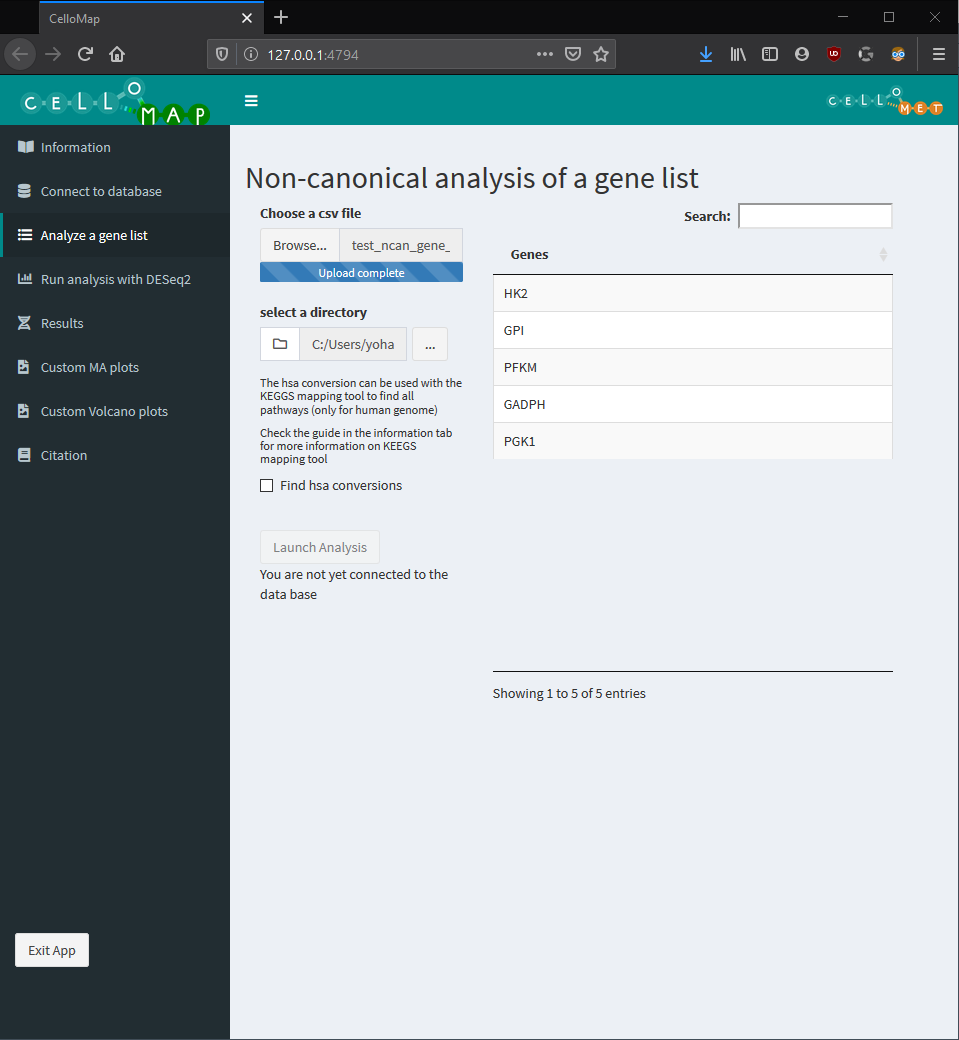
\includegraphics[width=15cm,height=10cm,keepaspectratio]{gene_list_analysis.png}
\caption{The gene list analysis tab once a correct file has been uploaded.}
\label{fig:gene_list_analysis_uploaded}
\end{figure}

Considering that the requirement for this analysis is a single column carrying the name `Genes', possible files to use are the significant gene list obtained from the \acrshort{DESeq2} analysis, or the significant differential expression results obtained from either the \acrshort{DESeq2} analysis or the downloading of the data from custom plots in \autoref{custom_plots}. A user could also create his own gene list file.
\subsection{KEGG Mapper \label{KEGG Map}}
By checking the `Find \acrshort{hsa} conversions' checkbox in the CelloMap tool, a conversion script will automatically be run along with a non-canonical gene analysis. This conversion will allow users to run a \acrshort{KEGG} mapping analysis using the file generated from the conversion.
\acrshort{KEGG} Mapper is a mapping tool that will search and find any pathways associated to a list of identifiers provided \cite{kanehisa2019kegg}. It will then allow the user to view every pathway found while highlighting the gene that was in the original list.
To perform the analysis, follow these steps, also seen in \autoref{fig:KEGG_mapper}.
IT is worth mentioning that the speed at which the conversion occurs depends on internet stability and speed as well as the amount of genes that need to be converted. It is recommended to have a stable internet connection to perform the \acrshort{hsa} conversion.
\begin{enumerate}
\item Go to the website: \url{https://www.kegg.jp/kegg/tool/map_pathway2.html}
\item Make sure that the search mode is \textbf{Organism-specific} with the letter \textbf{\acrshort{hsa}} in the text box
\item Upload the file created by CelloMap, the file will be called \textbf{\acrshort{hsa}\_ID.txt} 
\item Launch the analysis and wait a few seconds/minutes
\end{enumerate}

\begin{figure}[h!]
\centering
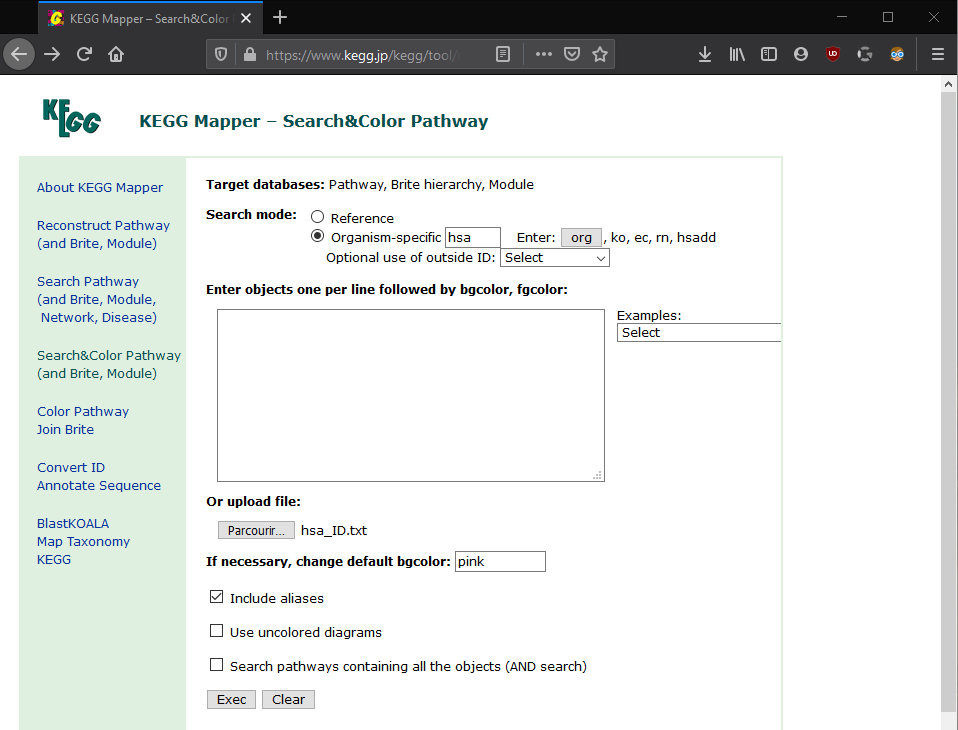
\includegraphics[width=15cm,height=10cm,keepaspectratio]{KEGG_Mapper.png}
\caption{The set-up for the \acrshort{KEGG} Mapper tool}
\label{fig:KEGG_mapper}
\end{figure}

\subsection{Metabolic GEne RApid Visualizer (MERAV)\label{MERAV}}
An alternative to the \acrshort{KEGG} Mapper is Metabolic GEne RApid Visualizer (\acrshort{MERAV}), this tool was designed to analyze \textbf{human} gene expression across a large variety of arrays. All of the arrays were normalized together to generate a gene expression database composed of several types of human tissue \cite{shaul2015merav}.
This tool offers two types of searches:
\begin{enumerate}
\item Search expression levels in one or several genes\\
This search will provide the user with the ability to search the database for the expression of a given gene(s).
\item Search all genes expression levels in one or more cell types\\
This search will provide the user with the ability to search the database for the expression of a given array.
\end{enumerate}

CelloMap creates a significant gene file that can be used with the first type of search, related to gene expression finding. To perform the search, follow these steps, also seen in \autoref{fig:merav}.
\begin{enumerate}
\item Go to the website: \url{http://merav.wi.mit.edu/}
\item Once on the website, click the `Search expression levels...' link.
\item Load the gene search box\\
To do this, copy paste all the genes from the significant gene file generated from \acrshort{DESeq2} or the one inputted in the gene list analysis. Do not include the line `Genes', as it will be considered a gene symbol and will not be found by the search tool. If it is included, it will not prevent the tool from searching for the other genes.
\item Set the parameters to your liking
\item If help is required, follow this link: \url{http://merav.wi.mit.edu/help/help.html}
\end{enumerate}

\begin{figure}[h!]
\centering
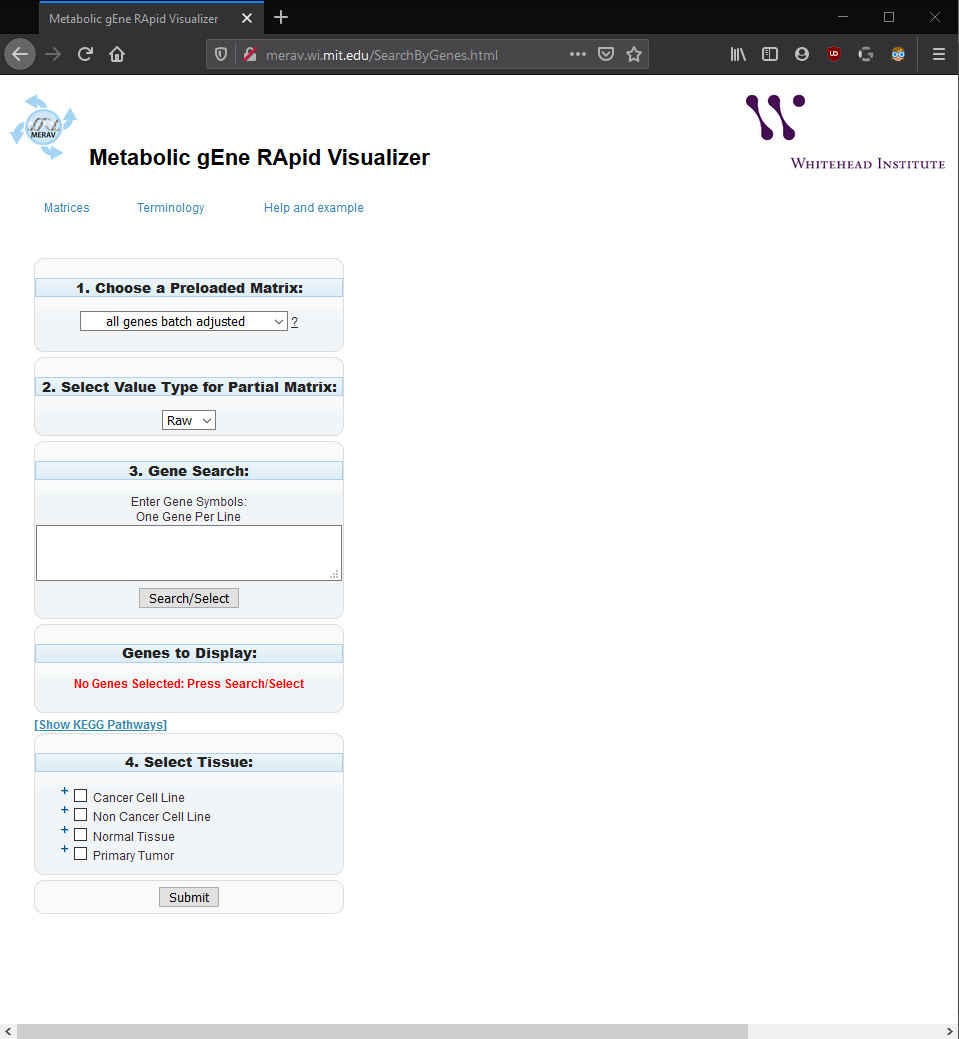
\includegraphics[width=15cm,height=10cm,keepaspectratio]{MERAV.png}
\caption{The set-up for the \acrshort{MERAV} search tool}
\label{fig:merav}
\end{figure}

\subsection{Non-canonical gene analysis}
The non-canonical analysis will cross check the provided gene list with our database, and if it finds non-canonical genes within the gene list, three text files will be created.
\begin{enumerate}
\item canonic\_results.txt\\
This file will contain the non-canonical gene symbols and names along with their \textbf{canonical} function and location.
\item non\_canonical\_results.txt\\
This file will contain the non-canonical gene symbols and names along with their \textbf{non-canonical} function and location.
\item references.txt\\
This file will contain the gene symbol and name of non-canonical genes and the references that were used to determine their canonical and non-canonical functions within this database.
\end{enumerate}
Each text file was created with the intention to be read by Microsoft excel. The text files need to be opened in excel and the separator/delimiter must be declared as `Tab'. Once opened, it is recommended to use the `wrap text' and `AutoFit Row Height' in the alignment and cell format sections of excel. This will ensure that the table is legible.


\section{Results \label{res}}
The results tab, seen in \autoref{fig:results_tab}, shows the results of a non-canonical gene analysis within the application itself. There isn't much to be said about this tab, it is only for visualization.
Every registered non-canonical genes are registered in a database hosted on Cellomet.com which can be accessed, updated and generally modified by the owner of Cellomet. For any questions regarding the non-canonical genes, their function, localization etc., please contact Cellomet via their website \cite{Cellomet}.

\begin{figure}[h!]
\centering
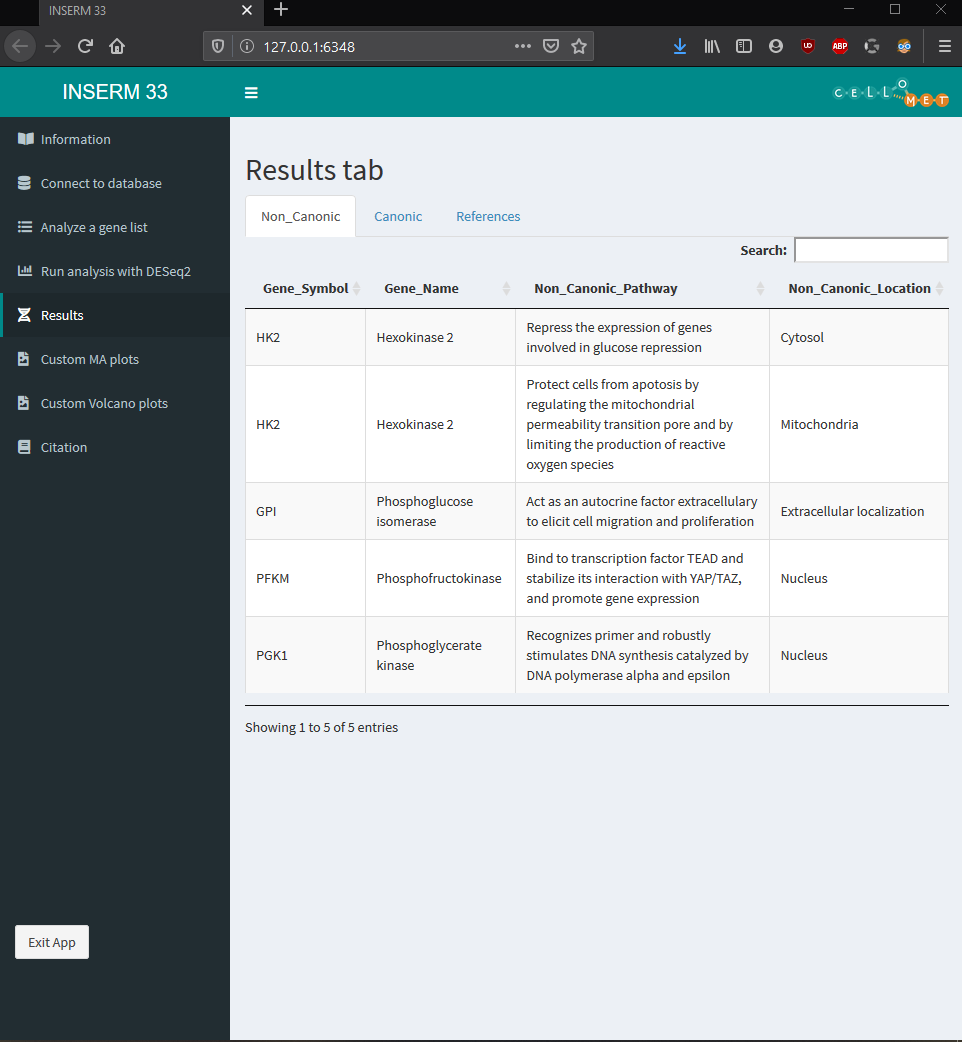
\includegraphics[width=15cm,height=10cm,keepaspectratio]{results_tab.png}
\caption{The results tab after a non canonical gene list analysis.}
\label{fig:results_tab}
\end{figure}


\section{Custom MA and Volcano plots \label{custom_plots}}
This application allows users to create their own custom figures, and from these figures, significant gene data can be downloaded. There are two possible figures, MA plots and Volcano plots \autoref{fig:maplot} and \autoref{fig:volcanoplot}, each plot type has it's own tab. However they behave very similarly, the volcano plot tab can be seen in \autoref{fig:custom_plots}. 
These tabs require a differential expression file, similar to those obtained from the \acrshort{DESeq2} analyses. The columns required are the `Genes' column, the `baseMean' column, the `log2FoldChange' column, the `pvalue' column, and the `\acrshort{Padj}' column, each written the same way as they are written in the guide. The file must also be a \acrshort{csv} file.
Aside that, each element of the different tabs is self explanatory. After each parameter modification, the `create plot' button needs to be clicked again. When a plot is loading, the rest of the application is locked to prevent the application from crashing due to a potential large number of buffered actions. For every modification in the parameters the plot must be re loaded before the modifications can be seen. Considering this, it is advised to have all the parameters set to your liking and re-load the plot with the `create plot' button. This is recommended as plots can take a few minutes to load depending on the computer and the size of the file.

\begin{figure}[h!]
\centering
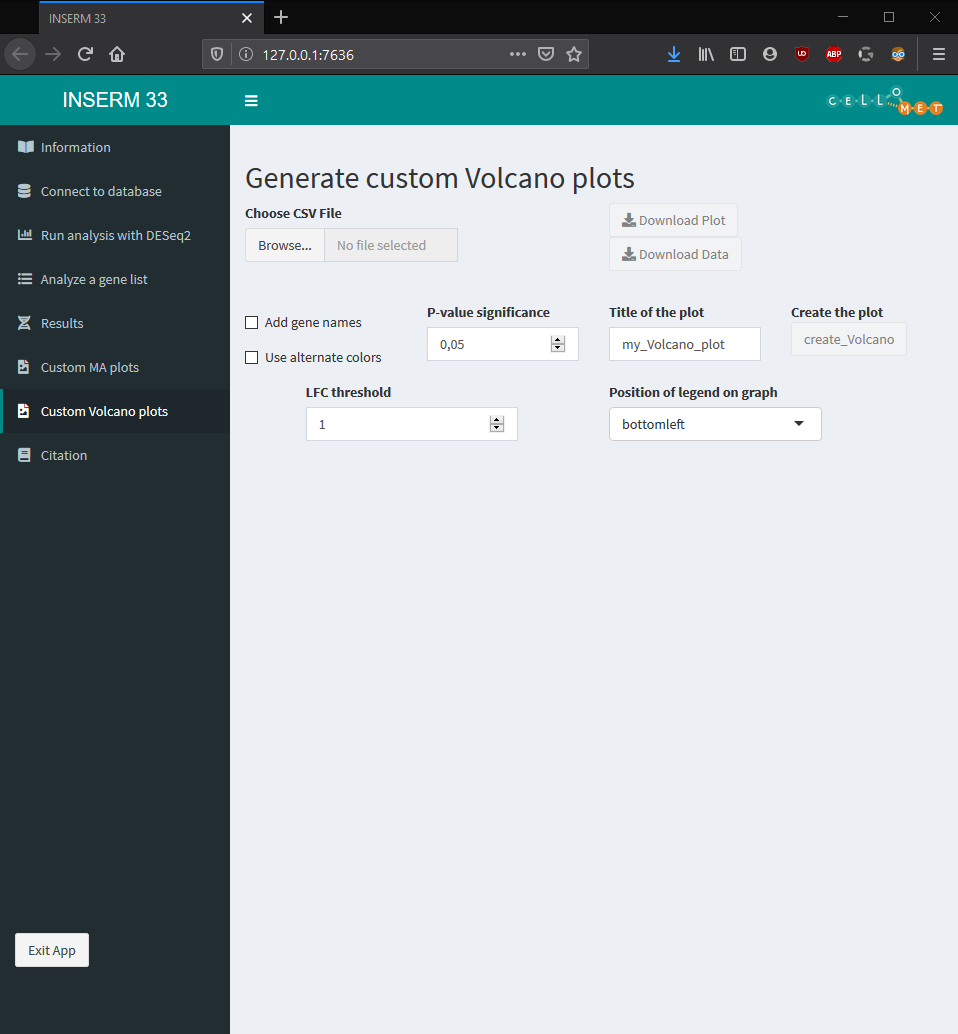
\includegraphics[width=15cm,height=10cm,keepaspectratio]{custom_volcano_tab.png}
\caption{The tab to create a custom volcano plot.}
\label{fig:custom_plots}
\end{figure}


\begin{figure}
    \centering
    \begin{minipage}{0.45\textwidth}
        \centering
        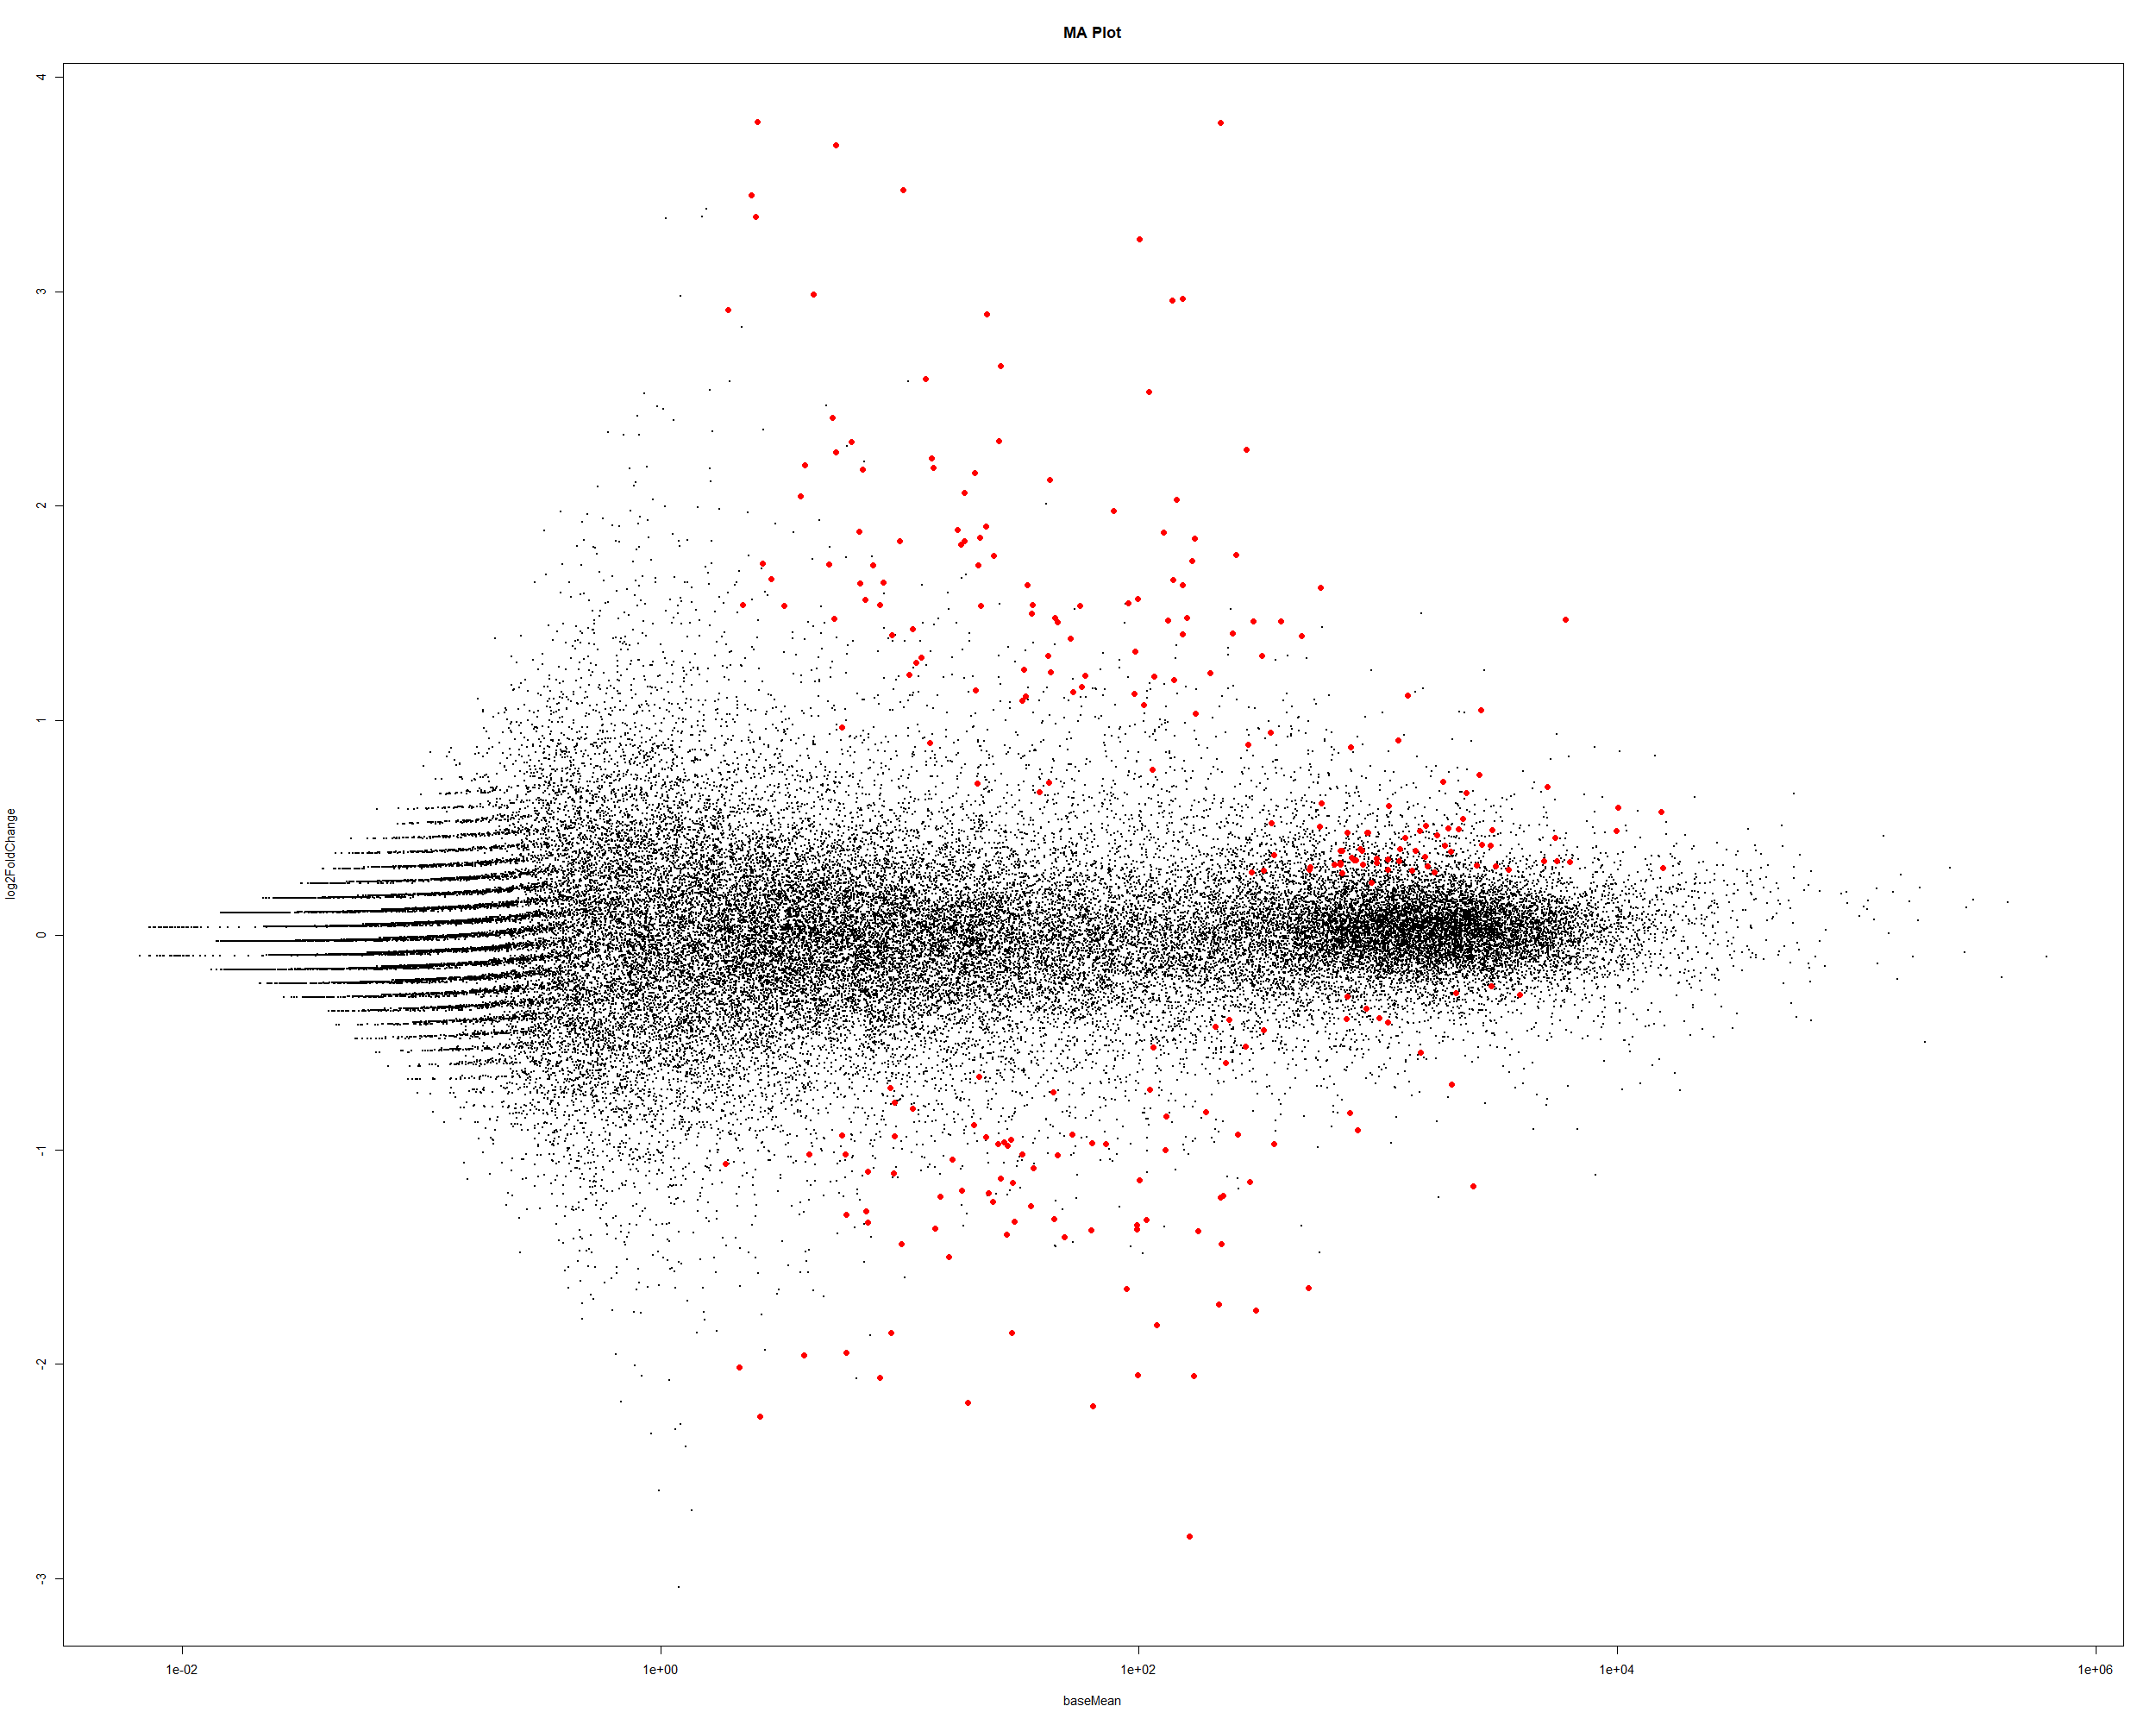
\includegraphics[width=1\textwidth]{maplot.png} % first figure itself
        \caption{An example of an MA plot with significant genes marked in red}
        \label{fig:maplot}
    \end{minipage}\hfill
    \begin{minipage}{0.45\textwidth}
        \centering
        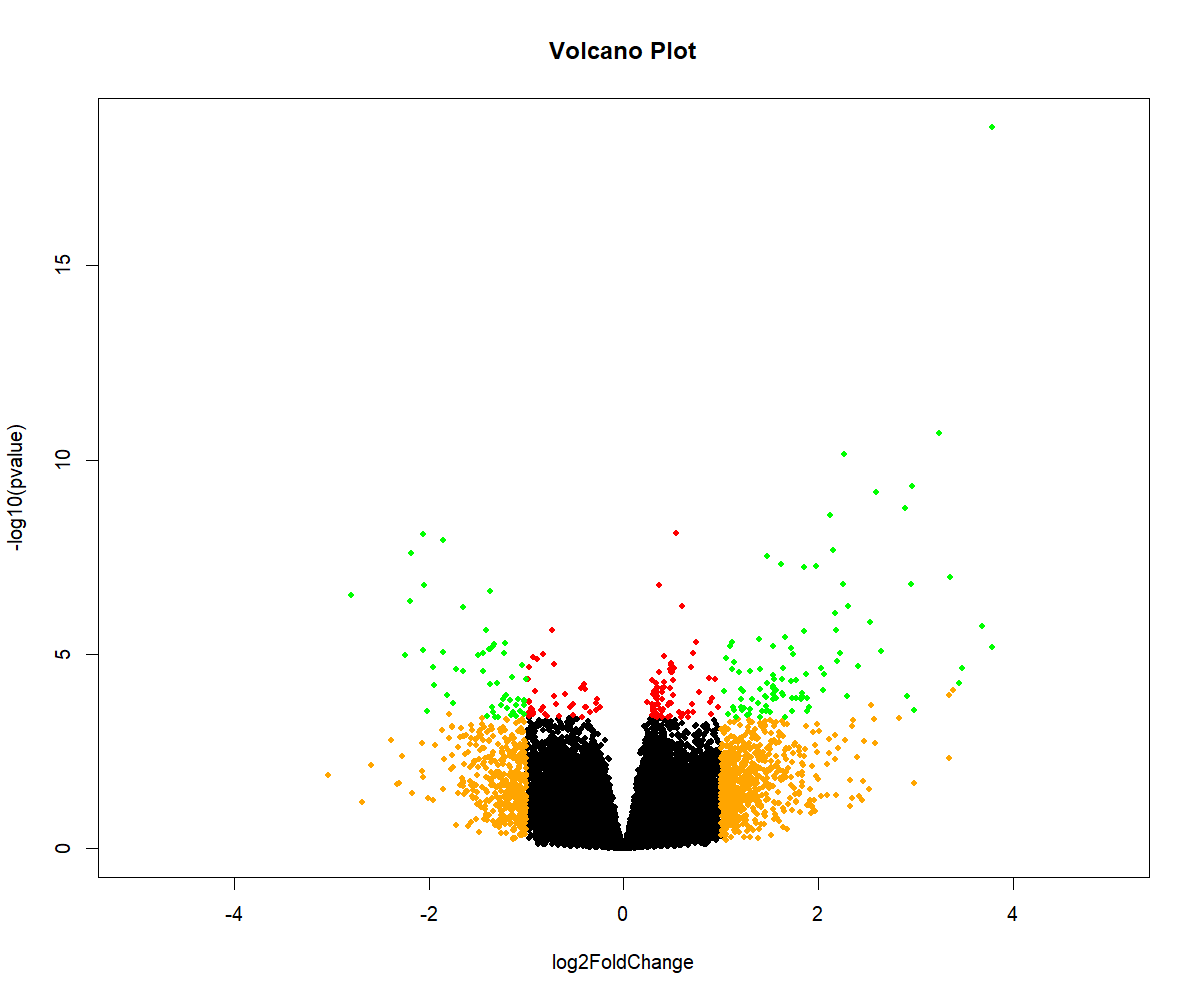
\includegraphics[width=1\textwidth]{volcano.png} % second figure itself
        \caption{An example of a volcano plot with significant genes marked in green}
        \label{fig:volcanoplot}
    \end{minipage}
\end{figure}



\section{Common errors \label{common_err}}
This section of the guide will cover possible errors that may be encountered and will be periodically updated if new errors are found. There errors either reflect actions, such as the inability to connect to the database, or actual error messages received in the error.txt file that may appear if an error occurred during an analysis.
\begin{enumerate}
\item \textbf{Failed to connect to database}\\
This may occur from time to time, the ideal is to wait and try again later. The database we are using has a limited number of connections at a time, as such, CelloMap was created in a way that it utilizes the connection as little as possible, by connecting right before it is needed and then removes the connection once it (the analysis) is done. This time frame lasts no more than ten minutes.
That said, if retrying several times has not solved the issue, it is recommended to contact one CelloMap's developer at the following email address: yohan.lefol@gmail.com.

\item \textbf{Error in DESeqDataSet(se, design = design, ignoreRank): design has a single variable, with all samples having the same value. use instead a design of `~ 1'. estimateSizeFactors, rlog and the VST can then be used}\\
This error may occur when only one condition is named, as well as randomly. It is a simple bug where \acrshort{DESeq2} finds only one variable and thus cannot proceed with its intended process.
To correct this issue, simply try again, make sure that two conditions are named and that both \acrshort{csv} files are properly uploaded to the application.
  
\end{enumerate}


\printglossary[type=\acronymtype]

\bibliographystyle{apacite}
\bibliography{references}
\end{document}